\documentclass[class=article, crop=false]{standalone}
\usepackage{tikz}
\usepackage{subcaption}
\usetikzlibrary{calc}

\begin{document}

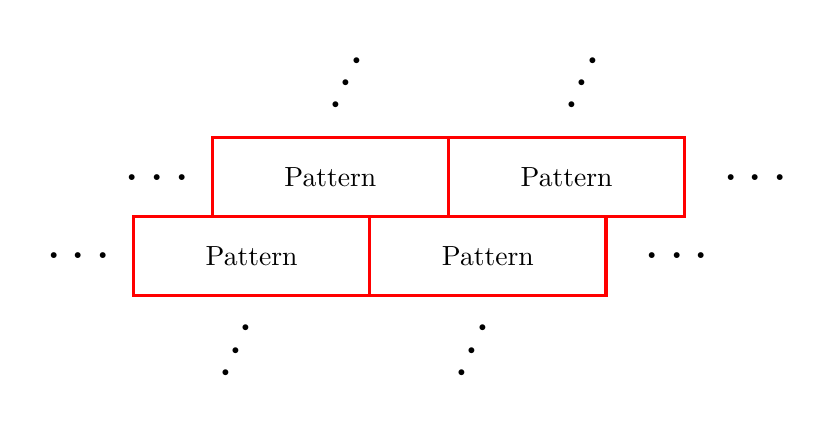
\begin{tikzpicture}
        % Add ellipses at start
        \node[scale=2] at (-0.2, .5) {$\ldots$};
        \node[scale=2] at (0.8, 1.5) {$\ldots$};
        \foreach \i in {0,...,1} {
            \foreach \j in {0,...,1} {
                \draw[red, very thick] (0.5+3*\i+\j,1*\j) rectangle (3.5+3*\i+\j,1*\j+1);
                \node at (2 + 3*\i+\j, 1*\j+.5) {Pattern};
        }}
        % Add ellipses at the end
        \node[scale=2] at (7.4, .5) {$\ldots$};
        \node[scale=2] at (8.4, 1.5) {$\ldots$};
        % Add ellipses above
        \node[scale=2,rotate=-115] at (3.2, 2.7) {$\ldots$};
        \node[scale=2,rotate=-115] at (6.2, 2.7) {$\ldots$};
        % Add ellipses below
        \node[scale=2,rotate=-115] at (1.8, -0.7) {$\ldots$};
        \node[scale=2,rotate=-115] at (4.8, -0.7) {$\ldots$};
    \end{tikzpicture}

\end{document}